\chapter{Theory}

Interactomic Potential Energy Surface (PES) is an important property of the
system
that enables us to explain and predict materials properties such as interfacial
energies, thermal expansion, cohesion, surface tension as well as chemical
reactions.
Representing PES accurately and efficiently is a major goal in molecular
modelling.
Existing approaches to PES modelling includes ab-initio models based on DFT,
empirical force fields fitted with experimental data, and the
relatively recent
machine learning based approach. The first one is accurate, parameter-free, and
transferable but has bad scaling with system size. The second one is
computationally efficient but has limited accuracy and transferability.
The third one combines both the advantages of the two previous approaches in
that it efficiently represents the PES for a
wide variety of systems with the level of accuracy of ab initio quantum
mechanics
models and scales for large systems.

% https://en.wikipedia.org/wiki/Interatomic_potential
This work will focus on a particular scheme for molecular modelling, the deep
neural network
potential molecular dynamics.

\section{Basics of Machine Learning}
Before dealing with deep potential molecular dynamics, one must have a basic
understanding on the principles of machine learning. Machine Learning (ML)
falls
under
the umbrella
term of Artificial Intelligence
(AI)
that focuses on developing algorithms that enable computers to learn from and
make decisions based on data. It is based on the idea that systems can
automatically improve their performance on a task through experience without
human intervention. The algorithm will understand the data by deconstructing it
in terms of hierarchy of concepts, with each concept defined through its
relation to simpler concepts. This allows the algorithm to learn complicated
concepts by building from simpler ones. Tasks such as classification,
regression, transcription, clustering, translation, to name a few can be solved
by ML \cite{Goodfellow2016}.


Regression learning works by allowing the program to fit an input of dimension
$\mathfrak{R}^n$ to an output of lower dimension $\mathfrak{R}^m$ by applying a
mapping function $f$.
Regression learning is an example of supervised learning since it
involves training a model on a labeled dataset. In practice, the labeled data
set is split into two: the training/learning and the testing/validation
data. The first one is feed to the algorithm while the second one is used to
validate the accuracy of the prediction.

Deep Learning is a type of ML that mimics the function of a
neuron in the living systems. It is divided into layers that constitutes the
input, output and multiple hidden layers where each layers contains collection
of
`neurons' or nodes as schematically shown in Figure \ref{fig:DL}. An algorithm
with one
hidden layer is
considered an Artificial Neural Network (ANN). Specifically, the algorithm is a
subset of Regression learning that maps an input to an output. Deep forwarded
network, also called
feed-forward neural network, refers to the idea that information moves in only
one direction from input, through the hidden layers,  to the output.  The goal
of a feedforward network is to approximate the mapping $y = f(x; w)$ of input
vector $x$ to an output vector $y$ by optimizing the values of the
parameters/weights $w$. Networking works by applying composition of many
different
functions. For a network with  $N$ layers depth, $N$ functions $f^1, f^2,
    \cdots, f^N$ will be
chained in succession to form $f(x) = f^N(\cdots f^2(f^1(x)))$. The innermost
function
refers to the first layer while the outermost function refers to the output
layer. Those functions that are in between refer to hidden layers since their
outputs are not desired.

% https://www.bmc.com/blogs/deep-neural-network/
\begin{figure}[h!]
    \centering
    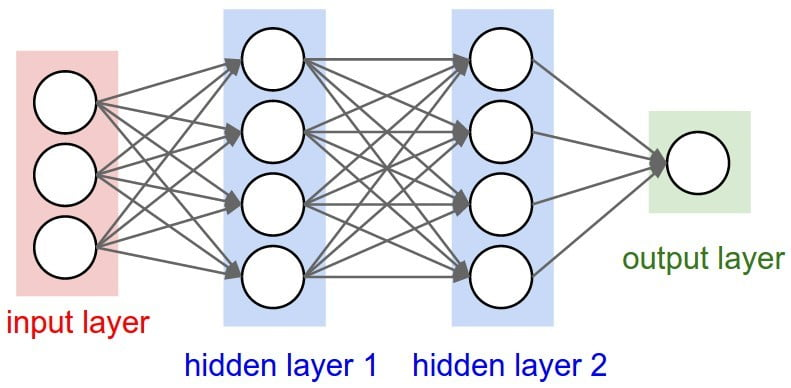
\includegraphics[width=0.5\linewidth]{images/DL.png}
    \caption{Typical configuration of a Deep Learning algorithm with 2 hidden
        layers that maps a $\mathfrak{R}^3$ input vector to a scalar output
        vector.}
    \label{fig:DL}
\end{figure}

To explain how each functions work, we look closely to the mathematical
interpretation of a neuron, as schematically shown in
Figure~\ref{fig:neuron_struc}. For a given artificial neuron $j$, let there be
$n+1$ inputs with signals $x_0$ through $x_n$ and weights $w_{0j}$ through
$w_{nj}$. The $x_0$ input is assigned the value +1, which makes it a bias input
with $w_{0j}$ = $b_j$. There will be $n$ actual inputs to the neuron: from
$x_1$ to $x_n$. The inputs will be weighted sum and the result is used as an
argument of the threshold function or activation function $\varphi$. Once the
function reaches a threshold value $\theta_j$ or more, it will give the output
or activation $a_j$ of the  $j$th neuron. Mathematically,

\begin{equation} \label{eq:activation_funct}
    a_j =   \varphi \left(\sum_{i=0}^{n} w_{ij}^T x_i \right) =  \varphi
    \left( z_{j}\right)
\end{equation}

Typical activation functions are Heaviside function, sigmoid, and rectified
linear functions (ReLu).

\begin{figure}[h!]
    \centering
    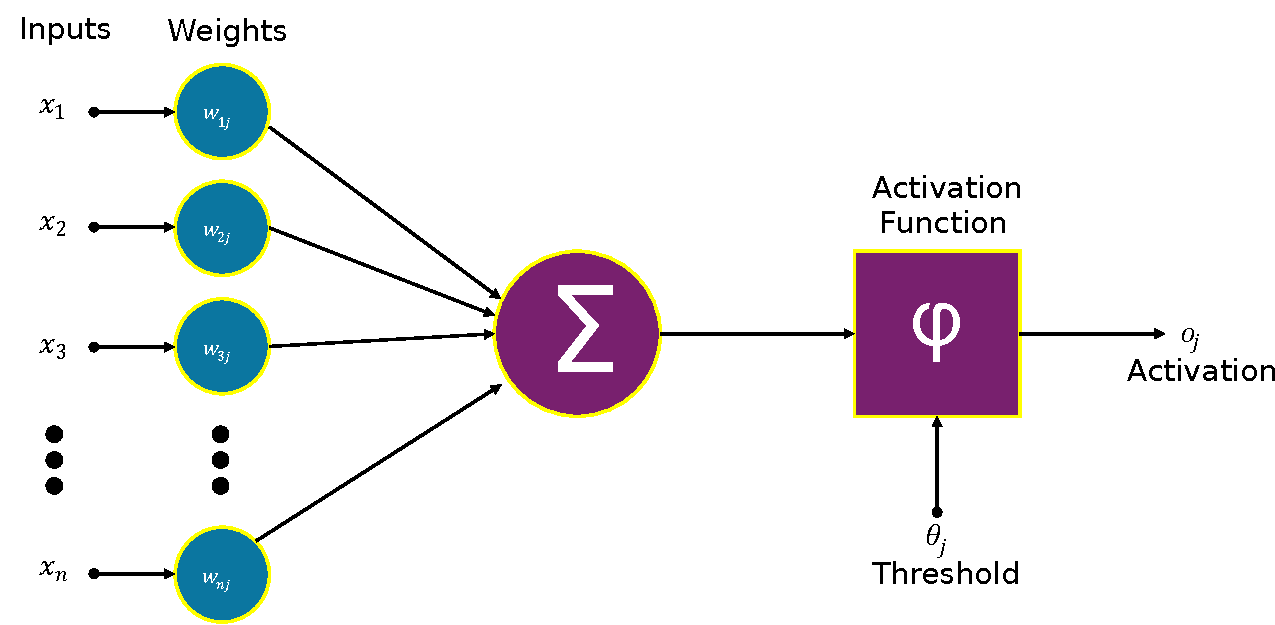
\includegraphics[width=0.5\linewidth]{images/artificial_neuron.pdf}
    \caption{The mathematical model of a neuron as first introduced by
        McCulloch and Pitts \cite{mcculloch1943logical}. Image taken at
        commons.wikimedia.org/wiki/File:Artificial\_neuron\_structure.svg}
    \label{fig:neuron_struc}
\end{figure}

One way to assess the performance of the training model is to compute the loss
function, or cost function, $\mathcal{L}$ with respect to the weights. A simple
choice is to compute the mean squared error
(MSE)
between the predicted $\hat{y}^{(\text{test})}$ and actual $y^{(\text{test})}$
value within the testing
dataset.

\begin{equation}
    \mathcal{L}^{(\text{test})}(w) = MSE^{(\text{test})} = \frac{1}{M} \sum_i^M
    \left(
    \hat{y}_i^{(\text{test})} -
    y_i^{(\text{test})} \right)^2  = \frac{1}{M} \sum_i^M
    \mathcal{L}^{(\text{test})}_i
\end{equation}

where $M$ is the number of test examples in the dataset. An algorithm should be
introduced to minimize the error  while allowing to gain
experience by incorporating a training dataset.
An intuitive way is to minimize the MSE on the training dataset with respect to
the weights by carrying out
the minimization problem called Gradient Descent

\begin{equation}
    \nabla_w \text{MSE}_\text{train} \approx 0
\end{equation}

The weights are updated by subtracting a factor proportional to the
gradient of the loss function.

\begin{equation}
    w_{n+1} = w_n - \epsilon  \grad_w \mathcal{L}(w)
\end{equation}

where $\epsilon$ is the learning rate and $n$ is the iteration step. Stochastic
Gradient Descent extends the well-known Gradient Descent algorithm. Instead of
computing the
actual gradient, which is computationally expensive for large training
datasets,  it is replaced
by an approximate gradient of a random subset of the training data. The loss
function is minimized by taking  the average gradient with respect to the
weights for $M'$ random minibatches of examples from the training set

\begin{align}
    \grad_w \mathcal{L}(w) \approx \frac{1}{M'} \sum_{i=1}^{M'} \grad_w L_i
\end{align}
where $L_i$ is the loss function of a specific training example $i$.

The stochastic gradient descent does a good job in reducing the computational
time, but the learning process can still be improved by implementing the
backpropagation algorithm. The algorithm works by computing the gradient of
the loss function with respect to each weights by utilizing chain rules in
backward fashion, from last layer to the first.

Without going to full derivation, the idea is to measure the sensitivity of the
loss function  to variations in  parameters such as weights,
biases and the activations.  For simplicity, consider the case of $N$ layers
with one neuron each. For one training example,  the loss function will be
$\mathcal{L}_0 = \left(a^{(N)} - y \right)^2$ where $a^{(N)}$ is the activation
of the
neuron at the last layer $N$ and $y$ is the actual value of the training
example. From eqtn.~\eqref{eq:activation_funct}, the activation will depend on
the previous layer

\begin{align}
    a^{(N)} & = \varphi \left( w^{(N)} a^{(N-1)} + b^{(N)} \right)
    \Longrightarrow
    \varphi
    \left( z^{(N)} \right)
\end{align}

where $w^{(N)}$ and $b^{(N)}$ are the weights and biases of the $N$th layer.
Taking relevant partial derivatives

\begin{align}
    \pdv{z^{(N)}}{w^{(N)}}       & = a^{(N-1)}, \quad \pdv{z^{(N)}}{b^{(N)}}
    =1,
    \quad \pdv{z^{(N)}}{a^{(N-1)}} = w^{(N)}                                 \\
    \pdv{a^{(N)}}{z^{(N)}}       & = \varphi'
    \left( z^{(N)} \right)                                                   \\
    \pdv{\mathcal{L}_0}{a^{(N)}} & = 2 \left(a^{(N)} - y \right)
\end{align}

By Chain Rule,

\begin{align}
    \pdv{\mathcal{L}_0}{w^{(N)}}		      =
    \pdv{\mathcal{L}_0}{a^{(N)}}
    \pdv{a^{(N)}}{z^{(N)}} \pdv{z^{(N)}}{w^{(N)}}    & = 2 \left(a^{(N)} - y
    \right)
    \varphi'
    \left( z^{(N)} \right)  a^{(N-1)}
    \\
    \pdv{\mathcal{L}_0}{a^{(N-1)}}		      =
    \pdv{\mathcal{L}_0}{a^{(N)}}
    \pdv{a^{(N)}}{z^{(N)}} \pdv{z^{(N)}}{a^{(N-1)} } & = 2 \left(a^{(N)} - y
    \right)
    \varphi'
    \left( z^{(N)} \right)  w^{(N)}
    \\
    \pdv{\mathcal{L}_0}{b^{(N)}}		      =
    \pdv{\mathcal{L}_0}{a^{(N)}}
    \pdv{a^{(N)}}{z^{(N)}} \pdv{z^{(N)}}{b^{(N)}}    & = 2 \left(a^{(N)} - y
    \right)
    \varphi'
    \left( z^{(N)} \right)
\end{align}

To generalize to more than one neurons per layer, one must introduce subscript
so that $a^{(N)}_j$ denotes the activation of  $j$th neuron in the $N$th layer
while $w^{(N)}_{jk}$ is the weight that connects the $j$th neuron in the $N$th
layer with the $k$th neuron in the previous layer. Also, define $z^{(N)}_j =
    \sum_k
    w^{(N)}_{jk} a^{(N-1)}_k + b^{(N)}_j$. The chain rule is modified as
follows

\begin{align}
    \pdv{\mathcal{L}_0}{w^{(N)}_{jk}} & =
    \pdv{\mathcal{L}_0}{a^{(N)}_j}
    \pdv{a^{(N)}_j}{z^{(N)}_j} \pdv{z^{(N)}_j}{w^{(N)}_{jk}}  =
    \pdv{\mathcal{L}_0}{a^{(N)}_j}
    \varphi'
    \left( z^{(N)}_j \right)  a^{(N-1)}_k
    \label{eq:back_prop1}
    \\
    \pdv{\mathcal{L}_0}{a^{(N-1)}_k}  & = \sum_{j=0}^{n_N-1}
    \pdv{\mathcal{L}_0}{a^{(N)}_j}
    \pdv{a^{(N)}_j}{z^{(N)}_j} \pdv{z^{(N)}_j}{a^{(N-1)}_k }  =
    \sum_{j=0}^{n_N-1} \pdv{\mathcal{L}_0}{a^{(N)}_j}
    \varphi'
    \left( z^{(N)}_j \right)  w^{(N)}_{jk}
    \label{eq:back_prop2}
    \\
    \pdv{\mathcal{L}_0}{b^{(N)}_j}    & =
    \pdv{\mathcal{L}_0}{a^{(N)}_j}
    \pdv{a^{(N)}_j}{z^{(N)}_j} \pdv{z^{(N)}_j}{b^{(N)}_j}     =
    \pdv{\mathcal{L}_0}{a^{(N)}_j}
    \varphi'
    \left( z^{(N)}_j \right)
\end{align}

Eqtn.~\eqref{eq:back_prop1} can be rewritten by using
eqtn.~\eqref{eq:back_prop2} for arbitrary layer $l$ as

\begin{equation}
    \pdv{\mathcal{L}_0}{w^{(l)}_{jk}} =  a^{(l-1)}_k \varphi'\left( z^{(l)}_j
    \right) \sum_{j=0}^{n_{l+1}-1}
    w^{(l+1)}_{jk} \varphi'
    \left( z^{(l+1)}_j \right)	 \pdv{\mathcal{L}_0}{a^{(l+1)}_j}
\end{equation}

This equation is  called the backpropagation formula where it got its name
since the error
of the
previous layer depends on the values of the forward layers. This formula
estimates the gradient that goes into updating the weights.

Deep learning continues to evolve rapidly, driven by advances in
computational power, availability of large datasets, and innovative algorithms.
It holds the promise of transforming various aspects of computational research
and industry
by enabling more intelligent autonomous systems.

\section{Deep Neural Molecular Dynamics}
Machine Learning potentials have very flexible functional form that allows to
represent reference data of quantum-mechanics accuracy at a cost that is
comparable to empirical force fields. Particularly, deep learning molecular
dynamics relies on using deep neural network trained potential (DeepPotential)
to simulate the
dynamics of the molecular system.  DeepPotential Method have basic assumptions
and features
\cite{zhang2018deep,zhang2018end},
namely

\begin{itemize}

    \item  Potential energy surface (PES) is extensive, it can be expressed as
          sum		of	     short-ranged many body atomic
          contributions
          \begin{equation}
              \Phi(\vec{r}_1,\vec{r}_1,\hdots, \vec{r}_N) = \sum_i
              \Phi_i(\{\mathcal{R}^i\})
          \end{equation}
          where $\Phi_i$ is represented by	     a		 function
          of atomic coordinates within the local environment of      the
          $i$th atom.
    \item  the function $\Phi_i$ is continuous and differentiable
          of atomic coordinates,
    \item the function $\Phi_i$ preserves the translational, rotational,
          and
          permutational symmetry of the system,
    \item the function $\Phi_i$ is represented from end-to-end by a deep
          neural network trained on DFT data
\end{itemize}

In regard to the first assumption, one can define first a global coordinate
matrix

\begin{equation}
    \mathcal{R} =  \mqty( x_1 & y_1 & z_1 \\ x_2 & y_2 & z_2 \\ \vdots & \ddots
    &
    \vdots \\
    x_N & y_N & z_N)
\end{equation}

that lists the absolute coordinates of all the $N$ atoms. Then, define a
relative
coordinate matrix of the local environment centered on atom  $i$ as

\begin{equation}
    \mathcal{R}^i =  \mqty( x_{1i} & y_{1i} & z_{1i} \\ x_{2i} & y_{2i} &
    z_{2i}
    \\ \vdots & \ddots
    &
    \vdots \\
    x_{N_i i} & y_{N_i i} & z_{N_i i})
\end{equation}

where $N_i$ are the number of atoms within the cutoff radius $r_c$ from the
central $i$th atom. Note that the coordinates are measured with respect to this
central atom, $\vec{r}_{ji} = \vec{r}_{j}- \vec{r}_{i}$. To impose smoothness
of the function, the relative coordinate matrix is mapped to  a renormalized
coordinate matrix

\begin{equation}
    \tilde{\mathcal{R}^i} =  \mqty( s(r_{1i}) &
    \frac{s(r_{1i}) x_{1i}}{r_{1i}}
    &	 \frac{s(r_{1i}) y_{1i}}{r_{1i}} &
    \frac{s(r_{1i}) z_{1i}}{r_{1i}} \\
    s(r_{2i}) &
    \frac{s(r_{2i}) x_{2i}}{r_{2i}}
    &	 \frac{s(r_{2i}) y_{2i}}{r_{2i}} &
    \frac{s(r_{2i}) z_{2i}}{r_{2i}}
    \\ \vdots & \vdots & \vdots
    &
    \vdots \\
    s(r_{N_i i}) &
    \frac{s(r_{N_i i}) x_{N_i i}}{r_{N_i i}}
    &	 \frac{s(r_{N_i i}) y_{N_i i}}{r_{N_i i}} &
    \frac{s(r_{N_i i}) z_{N_i i}}{r_{N_i i}} )
\end{equation}

where $s(r)$ is a smooth switching function defined as

\begin{equation}
    s(r) = \begin{cases}
        \frac{1}{r}                                   & , r   < r_s        \\
        \frac{1}{r} \left[x^3 (-6x^2+15x-10)+1\right] & , r_s \leq r < r_c \\
        0                                             & , r   \geq r_c
    \end{cases}
\end{equation}

where $x = \frac{r- r_s}{r_c-r_s}$, $r_c$ is the cutoff radius and $r_s$ is the
distance from atom $i$ where smoothing is applied. The	smooth cut-off
parameter $r_s$ allows the components of $\tilde{\mathcal{R}^i}$ to
go to zero smoothly at the boundary of the local region defined by $r_c$.
Particularly, the smoothing function $s(r)$ reduces the weight of atoms that
are farther from atom $i$, and at the same time removing the discontinuity
introduced by the cut-off. The renormalized coordinate matrix will serve as a
local descriptor that will feed into a specific deep neural network
NN$^{\alpha_i}$ where $\alpha_i$ is the chemical type of atom $i$. The output
of the neural network is the local atomic energy $\epsilon_i$ of the $i$th
atom. Then, the PES is given by the sum of the local atomic energies

\begin{equation}
    E = \sum_i^N	\epsilon_i
\end{equation}

while the atomic forces are

\begin{equation}
    \vec{F}_i = - \nabla_{\vec{R}_i} E = - \sum_i^N \nabla_{\vec{R}_i}
    \epsilon_i
\end{equation}

and the components of stress tensor is defined as

\begin{equation}
    \Xi_{\alpha \beta} = \sum_i^N R_{i\alpha} F_{i\beta}
\end{equation}

The training is performed with the stochastic descent method, minimizing the
loss function with respect to the weights of the deep neural network. The
evaluation of the gradient is carried out using backpropagation algorithm,
with the loss function defined as

\begin{equation}
    \mathcal{L} =   \frac{1}{M} \sum_l^M  \left[  p_E \left(\hat{E}^l- E^l
        \right)^2 +
        p_F \abs{\hat{\vec{F}}^l- \vec{F}^l}^2 + p_V \left(\hat{\Xi}^l- \Xi^l
        \right)^2 \right]
\end{equation}

where $M$ is the number of examples in the minibatch; $\hat{E}^l$,
$\hat{\vec{F}}^l$, and $\hat{\Xi}^l$
are the predicted energies, total forces, and stress tensor; $E^l$,
$\vec{F}^l$, and $\Xi^l$ are
the DFT
energies, forces, and stress tensor; $p_E$, $p_F$, and $p_V$  are tunable
prefactors
useful to improve the
efficiency of the training.